\documentclass[../probability-notes.tex]{subfiles}
\begin{document}
    \chapter{Limit Theorems}
    Here we look at inequalities around the mean (and variance) of random variables and try to get bounds on probabilities of certain associated events. These are especially useful when either the distribution of the random variable is not available, or calculating it may be difficult.

    %%%%%%%%%%%%%%%%%%%%%%%%%%%%%%%%%%%%%%%%%%%%%%%%%%%%%%%%%%%%%%%%%%%%%%%%%%%
    \section{Markov Inequality}
    For any non-negative random variable $X$ and positive $a$,
    \begin{align*}
        P(X \geq a) \leq \frac{E[X]}{a}
    \end{align*}
    This means that for a random variable with small mean, the probability of taking large values is small.\newline

    This can be proved as follows
    \begin{align*}
        E[X] &= \int_{0}^{\infty} xp_{X}(x) dx = \int_{0}^{a} xp_{X}(x) dx + \int_{a}^{\infty} xp_{X}(x) dx\\
        &\geq \int_{a}^{\infty} xp_{X}(x) dx \geq \int_{a}^{\infty} ap_{X}(x) dx = a\int_{a}^{\infty} p_{X}(x) dx\\
        &\geq aP(X \geq a)
    \end{align*}

    Based on experiments with simple distributions (like uniform distribution), it can be verified that the bounds provided this inequality can be quite loose.

    %%%%%%%%%%%%%%%%%%%%%%%%%%%%%%%%%%%%%%%%%%%%%%%%%%%%%%%%%%%%%%%%%%%%%%%%%%%
    \section{Chebychev Inequality}
    For any random variable $X$ with mean $\mu$ and variance $\sigma^{2}$, and a positive $k$,
    \begin{align*}
        P(\lvert X - \mu \rvert \geq k) \leq \frac{\sigma^{2}}{k^{2}}
    \end{align*}
    This means that for a random variable with small variance, the probability of taking a value far from the mean is small.\newline

    This can be proved using Markov's inequality on the non negative random variable $(X-\mu)^{2}$ and positive $k^{2}$
    \begin{align*}
        P((X-\mu)^{2} \geq k^{2}) &\leq \frac{E[(X-\mu)^{2}]}{k^{2}}\\
        \text{or, } \; P(\lvert X - \mu \rvert \geq k) &\leq \frac{\sigma^{2}}{k^{2}}
    \end{align*}

    Substituiting $k = c\sigma$,
    \begin{align*}
        P(\lvert X - \mu \rvert \geq c\sigma) \leq \frac{1}{c^{2}}
    \end{align*}


    %%%%%%%%%%%%%%%%%%%%%%%%%%%%%%%%%%%%%%%%%%%%%%%%%%%%%%%%%%%%%%%%%%%%%%%%%%%
    \section{Weak Law of Large Numbers}
    The weak law of large numbers provides bounds on the error between the true mean of a distribution and its estimated value from a sequence of random variables. Let $X_{1}, X_{2}, \ldots, X_{n}$ be a sequence of $n$ identically distributed random variables with mean $\mu$ and (a finite) variance $\sigma^{2}$, then
    \begin{align*}
        M_{n} &= \frac{X_{1} + \cdots + X_{n}}{n}\\
        P(\mid M_{n} - \mu \mid \geq \epsilon) &\leq \frac{\sigma^{2}}{n\epsilon^{2}}\\
        \lim_{n \to \infty} P(\mid M_{n} - \mu \mid \geq \epsilon) &\to 0
    \end{align*}

    For a distribution with finite variance, the above follows from Chebychev's inequality on $M_{n}$
    \begin{align*}
        M_{n} &= \frac{X_{1} + X_{2} + \cdots + X_{n}}{n} \\
        E[M_{n}] &= \frac{1}{n} \sum_{i=1}^{n} E[X_{i}] = \mu \text{\;\; expectation of expectation} \\
        Var(M_{n}) &= \sum_{i=1}^{n} Var(\frac{X_{i}}{n}) = \frac{\sigma^{2}}{n} \text{\;\; since $X_{i}$ are independent} \\
        \Aboxed{P(\mid M_{n} - \mu \mid \geq \epsilon) &\leq \frac{\sigma^{2}}{n\epsilon^{2}}}
    \end{align*}
    The above expression allows us to calculate the probability that $M_{n}$ falls in the interval $[\mu-\epsilon, \mu+\epsilon]$. As the value of $epsilon$ grows smaller, we will require a large value of $n$ to be able to confidently say that $M_{n}$ indeed falls in that range.\newline

    In cases where the true variance of the distribution is not known, we can still use the above inequality in the context of an upper bound on the variance. For instance, it can be shown that the variance of a $Bernoulli(p)$ is $p(1-p) \leq 1/4$.

    %%%%%%%%%%%%%%%%%%%%%%%%%%%%%%%%%%%%%%%%%%%%%%%%%%%%%%%%%%%%%%%%%%%%%%%%%%%
    \section{Convergence in Probability}
    First, we consider convergence in the context of a sequence of real numbers. A sequence of real numbers $a_{1}, a_{2}, \ldots$ converges to $a$ if for every $\epsilon > 0$, there exists $n_{0}$ such that $\lvert a_{n} - a \rvert \leq \epsilon$ for all $n \geq n_{0}$.\newline

    \subsection{Sequence of Random Variables}
    Before jumping to convergence in probability, lets review what a sequence of random variables represents. Consider a sample space $S = \{s_{1}, s_{2}, \ldots\}$. A random variable $X$ maps every outcome of the sample space to a real number and associates a probability to those real numbers: $X(s_{i}) = x_{i}$.\newline

    A sequence of random numbers will provide a different mapping that will be dependent on n: $X_{n}(s_{i}) = x_{n,i}$. When discussing convergence of a sequence of random variables, we will refer to a sequence of such kind. A basic example of such a sequence can be on a coin toss
    \begin{align*}
        X_{n} = \begin{cases} 1/(n+1) &\mbox{if Heads}\\ 1 &\mbox{if Tails} \end{cases}
    \end{align*}

    \subsection{Types of Convergence}
    There are different types of convergences. Some are stronger and others weaker. Stronger convergence can imply the weaker ones, but not the other way around.\newline
    The diagram below summarizes the relation between the different types of convergence. The convergences are arranged in decreasing order of strength from top to bottom.

    \begin{center}
    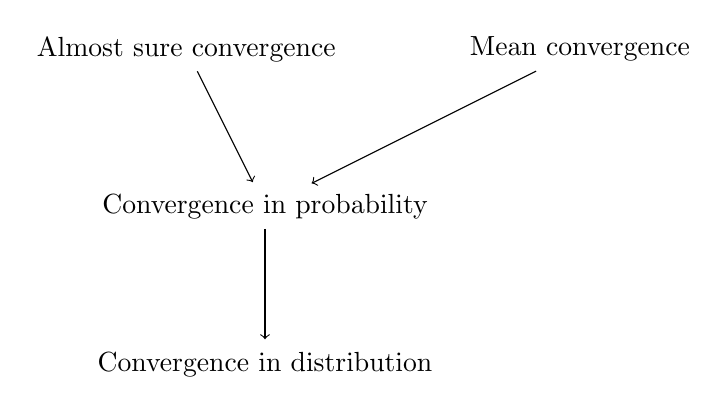
\begin{tikzpicture}
        % first add the node that we want to represent
        \node at (0,0)    (1) {Almost sure convergence};
        \node at (5,0)    (2) {Mean convergence};
        \node at (1,-2)    (3) {Convergence in probability};
        \node at (1,-4)    (4) {Convergence in distribution};
        % draw the edges between the nodes
        % bend left/right is from the persepective of the starting node
        % and so is the auto=left/right which specifies the side to put text
        \draw[every loop]
            % 1
            (1) edge (3)
            (2) edge (3)
            % 3
            (3) edge (4);
    \end{tikzpicture}
    \end{center}

    \subsubsection{Convergence in Distribution}
    This is the weakest type of convergence and only deals with the CDF. There is no requirement for $X_{n}$ to converge to $X$. Mathematically, A sequence of random variables $X_{i}$ converges in distribution to $X$ if for $\lim_{n \to \infty} P(X_{n} \leq x) = P(X \leq x)$ for all $x$ where $F_{X}(x) = P(X \leq x)$ is continuous. This is denoted as $X_{n} \overset{d}\rightarrow X$.\newline

    If $X_{i}$ and $X$ are both discrete distributions with non-negative integral values, then $X_{n} \overset{d}\rightarrow X$ if and only if $\lim_{n \to \infty} P_{X_{n}}(x) = P_{X}(x)$. This can be proved by first assuming LHS to be true to derive RHS and vice versa. With this, we can prove that a Bernoulli random variable converges to Poisson in the limit $n \to \infty$. CLT is a famous example of convergence in distribution and is discussed in subsequent sections.

    \subsubsection{Convergence in Probability}
    Convergence in probability is stronger than convergence in distribution. A sequence of random variables $X_{i}$ converges in probability to $X$ if for $\lim_{n \to \infty} P(\lvert X_{n} - X \rvert \geq \epsilon) = 0$ for every $\epsilon > 0$. This is denoted as $X_{n} \overset{p}\rightarrow X$.\newline

    We can also write this in similar terms as the convergence of a sequence of real numbers by changing the formulation. A sequence of random variables $X_{n}$ converges to $X$ if for every $\epsilon > 0$, there exists $n_{0}$ such that $P(\lvert X_{n} - X \rvert \geq \epsilon) \leq \delta$ for all $n \geq n_{0}$.\newline

    A famous example of this type of convergence is the weak law of large numbers discussed earlier.

    \subsubsection{Convergence in Mean}
    For a fixed $r \geq 1$, a sequence of random variables $X_{i}$ is said to converge to $X$ in the $r^{th}$ mean or in the $L^{r}$ norm if $\lim_{n \to \infty} E[\lvert X_{n} - X \rvert^{r}] = 0$. This is denoted by $X_{n} \overset{L^{r}}\rightarrow X$. For $r=2$ this is called mean-square convergence and is denoted by $X_{n} \overset{m.s.}\rightarrow X$.\newline

    Mean convergence is stronger than convergence in probability, i.e., convergence in $L^{r}$ norm implies convergence in probability as well.

    \subsubsection{Almost Sure Convergence}
    Consider a sequence of random variables $X_{1}, X_{2}, X_{3}, \ldots$ defined on a sample space $S$ (assume finite for the moment) $= \{s_{1}, s_{2}, \ldots s_{k}\}$. Since a random variable $X_{n}$ is a mapping from an outcome in sample space to the set of real numbers, $X_{n}(s_{i}) = x_{ni}$ for $i=1,2,\ldots,k$.\newline

    After performing the random experiment, one of the $s_{i}$\'s will be the outcome of the experiment and we will know the value for all the $X_{n}$\'s. For $s_{j}$ as the outcome, we observe the sequence $x_{1j}, x_{2j}, \ldots$. Almost surely convergence is defined based on the convergence of this sequence of numbers.\newline

    A sequence of random variables $X_{1}, X_{2}, \ldots$ converges almost surely to a random variable $X$ if $P(\{s \in S:\lim_{n \to \infty} X_{n}(s) = X(s)\}) = 1$ and is denoted by $X_{n} \overset{a.s.}\rightarrow X$.\newline

    There is a useful results to show almost convergence. If for the sequence of random variables and all $\epsilon > 0$, we have
    \begin{align*}
        \sum_{n=1}^{\infty}P(\lvert X_{n} - X \rvert > \epsilon) &< \infty\\
        \implies X_{n}(s) &= X(s)
    \end{align*}
    This is only a sufficient condition. Below is a condition that is both necessary and sufficient
    \begin{align*}
        A_{m} = \{\lvert X_{n} - X \rvert < \epsilon \;\text{for all}\; n \geq m \}\\
        \text{Then, }\; X_{n} \overset{a.s.}\rightarrow X \;\text{if and only if for any $\epsilon > 0$}\\
        \lim_{m \to \infty} P(A_{m}) = 1
    \end{align*}
    A famous theorem in almost surely convergence is the strong law of large numbers, which states that for a set of independent identically distributed random with a finite mean, the expected value of the average of the random numbers almost surely converges to the mean.

    \subsubsection{Continuous Mapping Theorems}
    Let $X_{1}, X_{2}, X_{3}, \ldots$ be a sequence of random variables, and let $h: \mathcal{R} \rightarrow \mathcal{R}$, then
    \begin{align*}
        \text{If}\; X_{n} \overset{d}\rightarrow X \; &\text{then} \; h(X_{n}) \overset{d}\rightarrow h(X)\\
        \text{If}\; X_{n} \overset{p}\rightarrow X \; &\text{then} \; h(X_{n}) \overset{p}\rightarrow h(X)\\
        \text{If}\; X_{n} \overset{a.s.}\rightarrow X \; &\text{then} \; h(X_{n}) \overset{a.s.}\rightarrow h(X)
    \end{align*}

    %%%%%%%%%%%%%%%%%%%%%%%%%%%%%%%%%%%%%%%%%%%%%%%%%%%%%%%%%%%%%%%%%%%%%%%%%%%
    \section{Central Limit Theorem}
    Chebychev's inequality gives a loose bound. We can do better with CLT. Let $X$ be a random variable with mean $\mu$ and variance $\sigma^{2}$, and let $X_{i}$ be independent identically distributed random variables with the same distribution as $X$. Consider the random variable $S_{n}$ defined below,
    \begin{align*}
        S_{n} &= X_{1} + X_{2} + \cdots + X_{n}\\
        Z_{n} &= \frac{S_{n} - E[S_{n}]}{\sigma_{n}} \text{\;\;random variable with mean $0$ and variance $1$} \\
             &= \frac{S_{n} - nE[X]}{\sqrt{n} \sigma}\\
        \text{Then,\;\;} \Aboxed{\lim_{n \to \infty} P \bigg(\frac{S_{n} - n\mu}{\sqrt{n} \sigma} \leq c \bigg) &= P(Z \leq c) = \Phi(c)}
    \end{align*}
    Or, the cumulative distribution of the random variable $(S_{n} - n\mu)/\sqrt{n} \sigma$ converges to that of a standard normal.\newline
    By defining the confidence on how close we desire $S_{n}$ to the actual mean, we can calculate the required value of the $n$ using standard normal CDF tables. However, we need to have an estimate of variance of the distribution in order to estimate $n$.\newline

    As a rule of thumb, $n=30$ gives a very close approximation to the normal distribution.\newline

    Similar to the weak law of large numbers, if the variance is not available, but an upper bound on the same can be obtained, the probability of intereset can be calculated using this bound.

    \subsection{De Moivre-Laplace Approximation to the Binomial}
    A Binomial random variable $S_{n}$ can be viewed as the sum of $n$ Bernoulli random variables $X_{i}$ with the parameter $p$. We can apply the central limit theorem to obtain the probabiliy of the variable between any two ranges
    \begin{align*}
        P(k \leq S_{n} \leq l) &= P(\frac{k - np}{\sqrt{n} p(1-p)} \leq \frac{S_{n} - np}{\sqrt{n} p(1-p)} \leq \frac{l - np}{\sqrt{n} p(1-p)})\\
        &= P(\frac{S_{n} - np}{\sqrt{n} p(1-p)} \leq \frac{l - np}{\sqrt{n} p(1-p)}) - P(\frac{S_{n} - np}{\sqrt{n} p(1-p)} \leq \frac{k - np}{\sqrt{n} p(1-p)})\\
        &\approx \Phi(\frac{l - np}{\sqrt{n} p(1-p)}) - \Phi(\frac{k - np}{\sqrt{n} p(1-p)}) \; \text{for large $n$}
    \end{align*}
    Since $S_{n}$ will take discrete values, $P(S_{n} <= k) = P(S_{n} < k+1)$ for any positive integer $k$. A better approximation of the above formula can be obtained by considering the middle point of $k$ and $k+1$ as applicable
    \begin{align*}
        P(k \leq S_{n} \leq l)&\approx \Phi(\frac{l + \frac{1}{2} - np}{\sqrt{n} p(1-p)}) - \Phi(\frac{k - \frac{1}{2} - np}{\sqrt{n} p(1-p)}) \; \text{for large $n$}
    \end{align*}

    This correction yields a more closer result to the actual values. With $p$ close to $1/2$, the approximation works well for $n = 40,50$ itself. The distribution is also symmetric at this point which helps the CLT.  However, as the $p$ becomes closer to $0$ or $1$, larger values of $n$ are required for the approximation to be valid.\newline

    We can also calculate the value of a single point as given below
    \begin{align*}
        P(S_{n} = k)&\approx \Phi(\frac{k - \frac{1}{2} - np}{\sqrt{n} p(1-p)}) - \Phi(\frac{k + \frac{1}{2} - np}{\sqrt{n} p(1-p)}) \; \text{for large $n$}
    \end{align*}


    %%%%%%%%%%%%%%%%%%%%%%%%%%%%%%%%%%%%%%%%%%%%%%%%%%%%%%%%%%%%%%%%%%%%%%%%%%%
    \section{Strong Law of Large Numbers}
    This law is similar to the weak law, but deals with the convergence of the mean. Let $X_{i}$ be $n$ independent identically distributed random variables with mean $\mu$. Then the mean $M_{n}$,
    \begin{align*}
        \lim_{n \to \infty} P(M_{n} = \mu) = 1
    \end{align*}

    That is, $M_{n}$ converges to $\mu$ with probability $1$ or \textbf{almost surely}. Convergence with probability $1$ implies convergence in probability, but the converse is not always true.\newline

    There is a subtle differnce between WLLn and SLLN. WLLN states that the probability of deviation of $M_{n}$ from the true mean is always finite, although the probability of deviation converges to $0$ in the limit. On the other hand, SLLN states with absolute certainty that in infinite experiments, the sample mean will converge to the true mean with probability $1$.
\end{document}
